%A Michelson interferometer converts a change in optical path length into a change in intensity of light. Shot noise is one of the fundamental limits on how precisely the path length can be known. As shot noise manifests as intensity fluctuations of the light, it is indistinguishable from intensity fluctuations that arise due to the differential phase modulation of interfering beams.
%\par
In this Chapter, it is demonstrated that the shot noise measured with the transimpedance amplifier developed for some of the experiments in Chapter~\ref{chapter:2um_photoiode_chapter} can be used to measure shot noise within an interferometer, thus linking the shot noise of a current to the phase of light. To do this, a Mach-Zehnder interferometer was used. This also makes the experiment topologically similar to a Michelson interferometer with a balanced homodyne detection scheme. A shot noise limited measurement was made in-air, and this is reported in Section~\ref{sec:MZ_chapter_in_air}. Section~\ref{sec:MZ_chapter_in_vac} is a description of an attempt to perform this measurement in-vacuum so that shot noise could be measured at lower frequencies, however due to scattered light, this was unsuccessful.
\section{Shot Noise in a Mach-Zehnder Interferometer}
\label{sec:MZ_chapter_in_air}
A sketch of a Mach-Zehnder interferometer is shown in Figure~\ref{fig:mzchaptermzsketch}. At the second beam splitter, two beams are combined to produce an interference pattern that depends on the relative phase between the two beams. This is analogous to an interferometer that uses balanced homodyne detection. In an interferometer with a balanced homodyne detection scheme, the two beams are called the signal and local oscillator.
\par
The difference between a Mach-Zehnder interferometer and a Michelson interferometer with a balanced homodyne detection scheme is what the phase of the signal beam means. In a Mach-Zehnder interferometer, the phase corresponds to the motion of a mirror whereas in a Michelson interferometer with a balanced homodyne detection scheme, the phase corresponds to a differential motion of the ETMs.
\begin{figure}
	\centering
	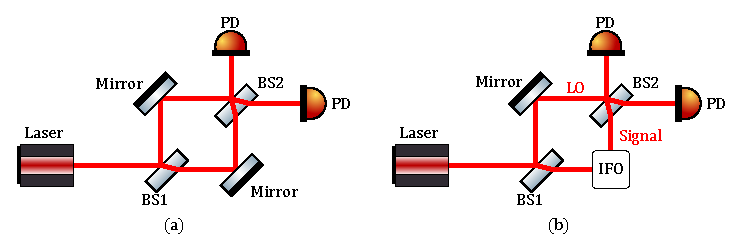
\includegraphics[width=1\linewidth]{Figures/MZ_chapter_mz_sketch}
	\caption{(a) Sketch of a Mach-Zehnder interferometer. The interference at BS2 depends on the difference in the phase of the two beams after BS1. (b) Sketch of an interferometer (IFO) with a balanced homodyne detection scheme. A Michelson interferometer adds a phase modulation to the signal beam, and this results in an intensity modulation in the combined beams after BS2. In essence, (b) is similar to (a).}
	\label{fig:mzchaptermzsketch}
\end{figure}
\par
The signal measured by each photodiode can be described by Equation (\ref{eq:bhdforligo_interference_at_a_beam_splitter}). The shot noise of this measurement depends on the total amount of light in the signal and LO beam, and because the power of the LO beam, $P_{\rm{LO}}$, was much greater than the power of the signal beam, $P_{\rm{sig}}$, the amplitude spectral density associated with the shot noise, $n_z$, of the detected light can be expressed in units of $\si{\metre_{\rm{rms}}/\sqrt{\hertz}}$ by
\begin{equation}
n_z = \sqrt{\frac{2hc\lambda}{16\pi^2P_{\rm{sig}}}}
\label{eq:MZ_chapter_shot_noise_level}.
\end{equation}
The noise, $n_z$, can be interpreted as the detected amount of relative motion between the two mirrors in the Mach-Zehnder interferometer. 
\subsection{Apparatus for the In-Air Mach-Zehnder.}
The in-air Mach-Zehnder is shown in Figure \ref{fig:mzchapterinairmz} and Figure \ref{fig:mzchapterinairsketch}. It was constructed from highly stable, rigid mounts to keep the noise due to the vibration of the mounts low. The Mach-Zehnder was mounted on a thick aluminium base-plate which was isolated from the optical table by rubber dampeners. The Mach-Zehnder was acoustically shielded with a plastic box of a $\sim1\si{\milli\metre}$ thickness. A half-wave plate and polarised beam splitter were used to control the power entering the Mach-Zehnder and the polarisation of the light entering the Mach-Zehnder.
\begin{figure}
	\centering
	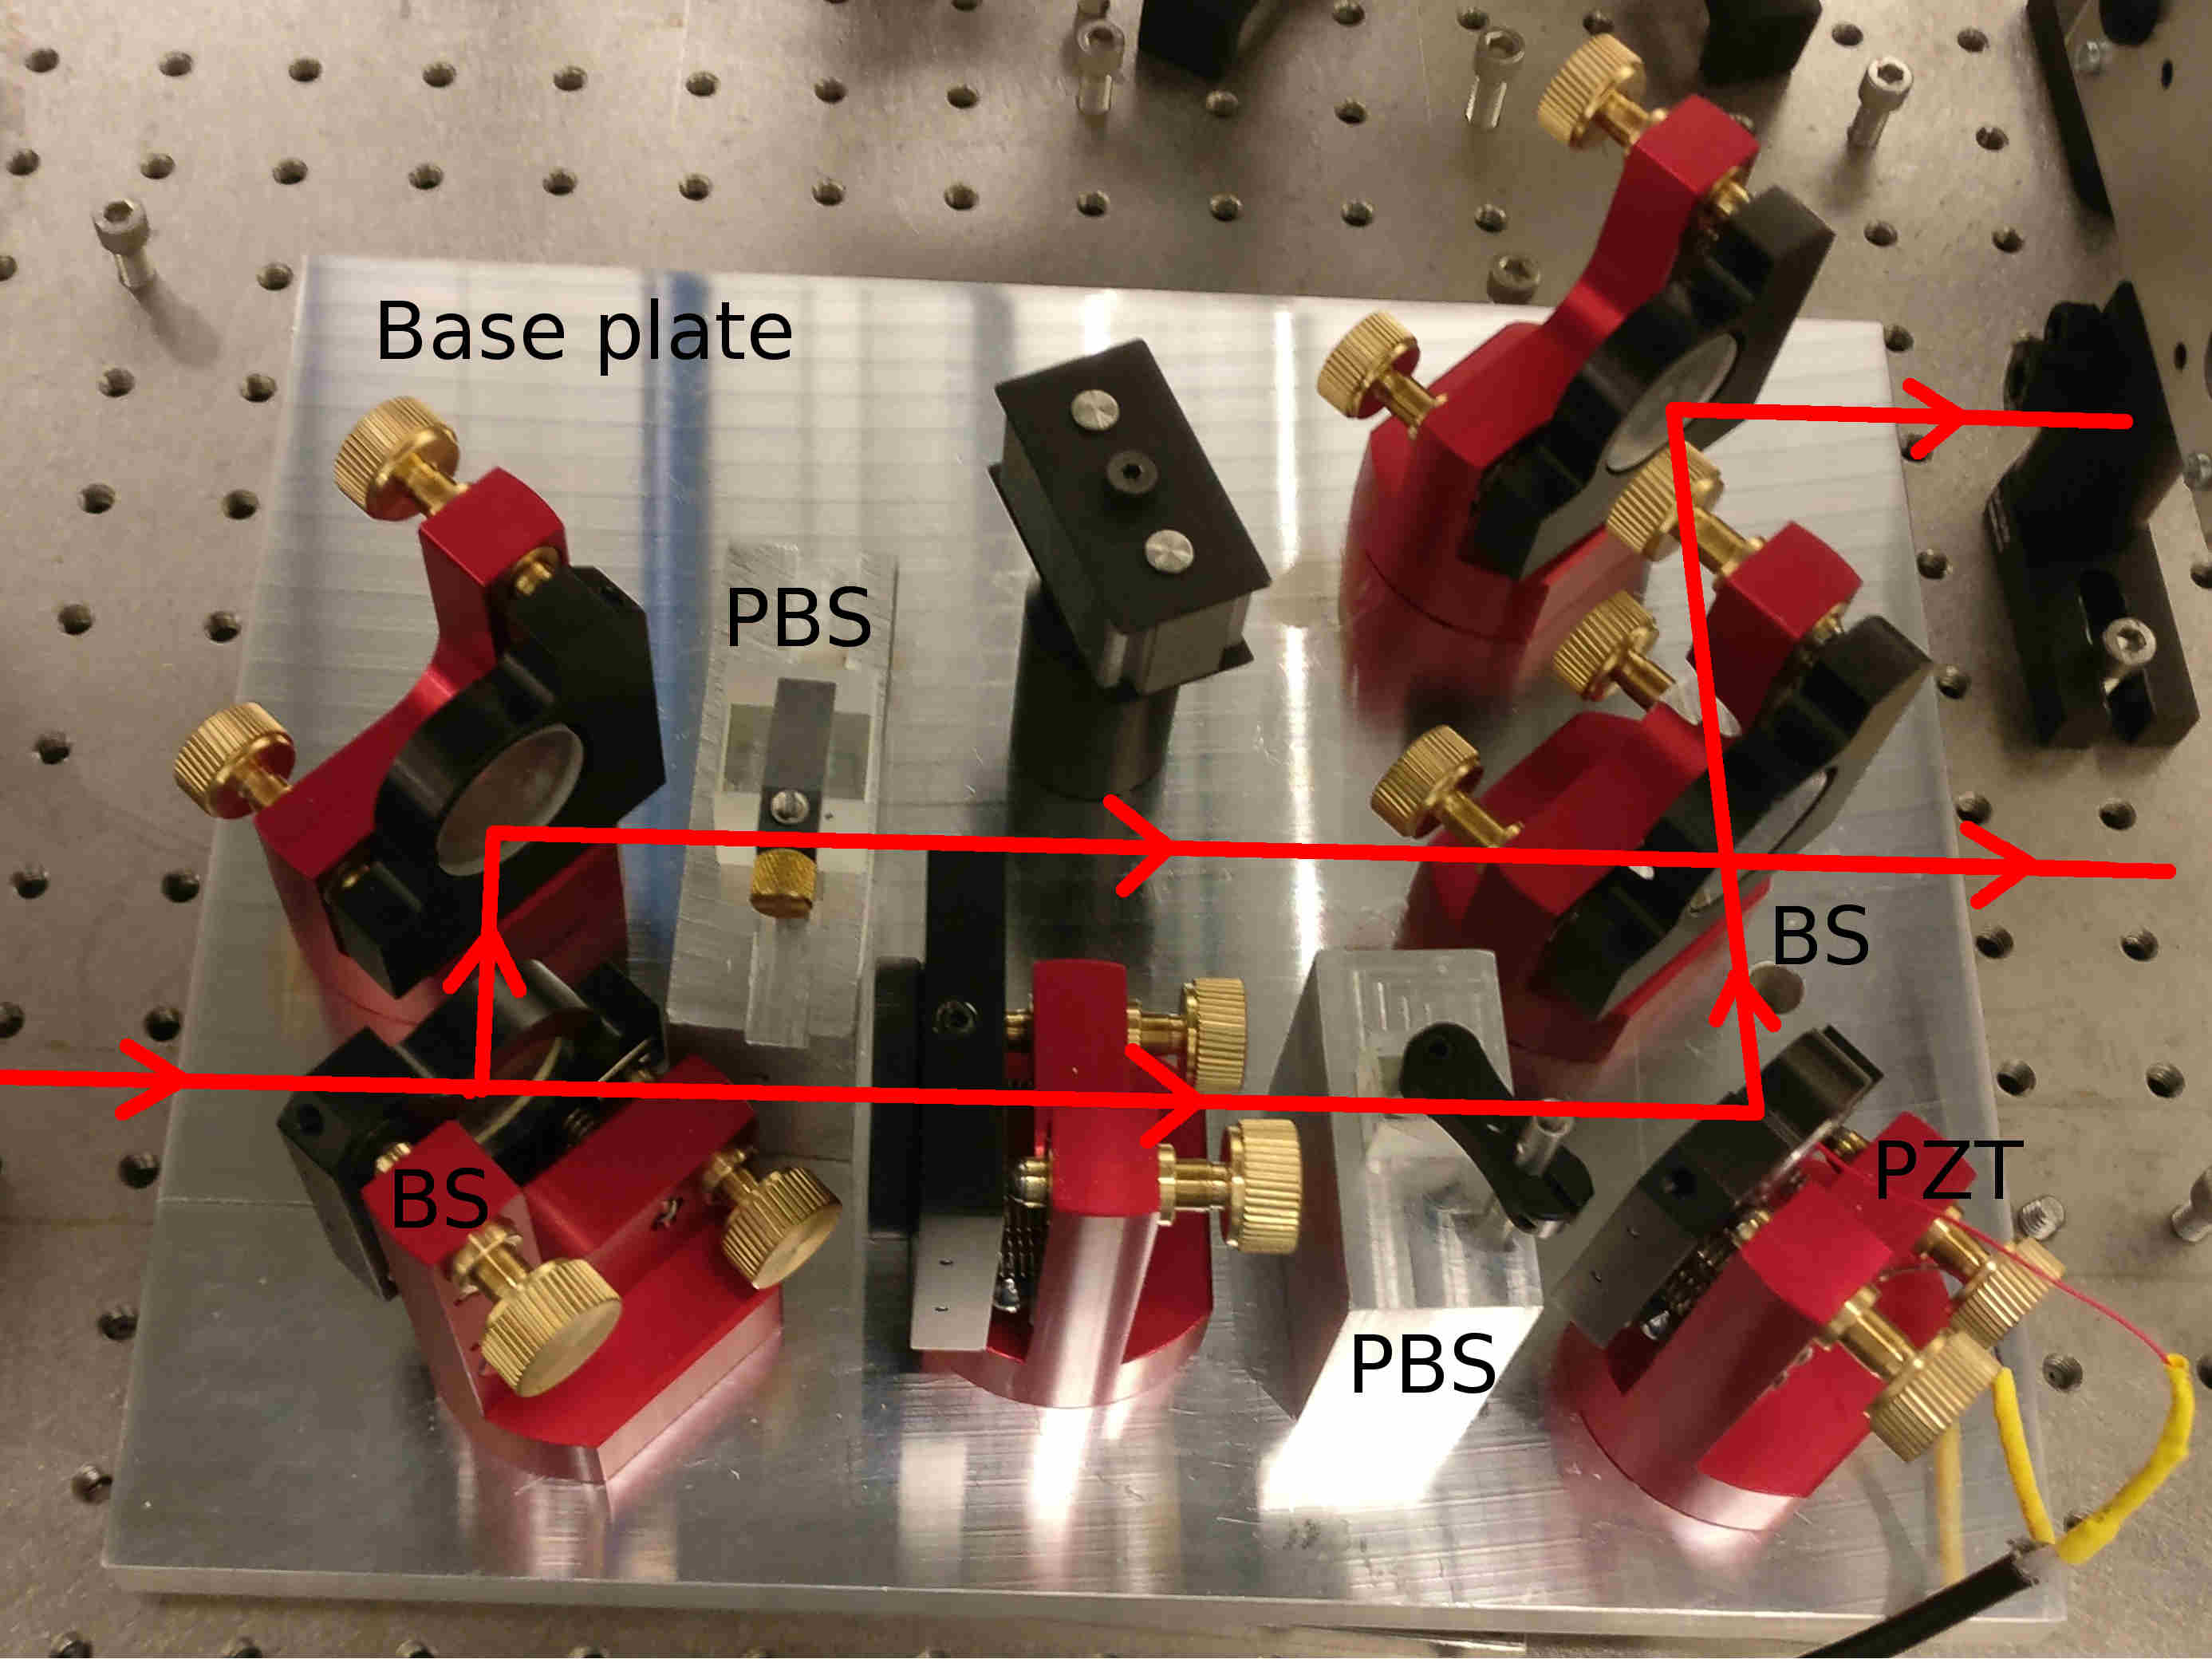
\includegraphics[width=0.7\linewidth]{Figures/MZ_chapter_in_air_MZ}
	\caption{Photograph of the Mach-Zehnder base plate. The polarising beam splitters were part of an earlier design; they were removed when the measurements with this apparatus were made. }
	\label{fig:mzchapterinairmz}
\end{figure}
\begin{figure}
	\centering
	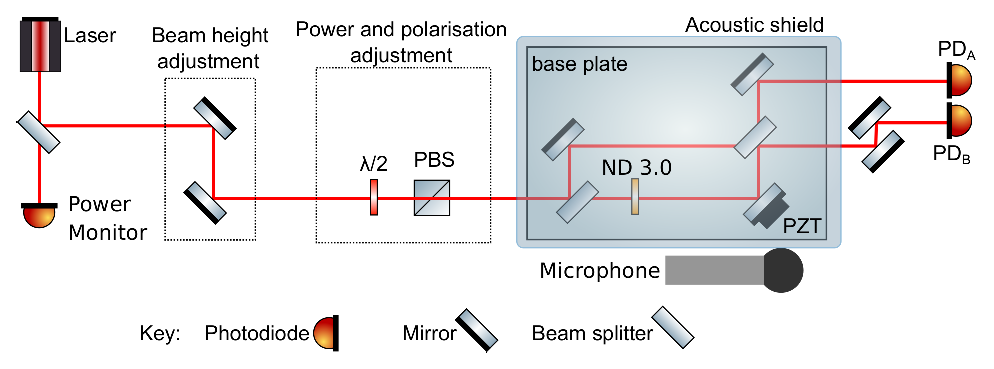
\includegraphics[width=1\linewidth]{Figures/MZ_chapter_in_air_sketch}
	\caption{Sketch of the optical layout. The laser was generated by an NPRO. The power of the laser was monitored using a photodiode immediately after the laser. The beam's power and polarisation were controlled with a half wave plate and polarising beam splitter (PBS). The Mach-Zehnder was mounted on a base plate, and it was acoustically shielded by a plastic box and rubber feet. The splitting ratio of the BS2 was measured to be 50:50. An ND filter was used to decrease the power in one of the paths within the Mach-Zehnder. }
	\label{fig:mzchapterinairsketch}
\end{figure}
\par
The reflectivity, $R$ and transmissivity, $T$, of the beam splitter on which the beams were recombined was measured to be $0.5\pm0.01$. To replicate a situation analogous to a balanced homodyne detection scheme, the power in one arm was attenuated. The beam size within the Mach-Zehnder was small, so the light power in one arm was attenuated with an ND filter as surface roughness of the ND filter did not matter. The optical density of the ND filter was found by measuring the ingoing and outgoing beam's power with $\rm{PD_A}$ and $\rm{PD_B}$; this was done by blocking the upper path and measuring the signal with and without the ND filter. The ND filter decreased the power in the signal arm by a factor of 232.
\par
The signals from the photodiodes were measured using the same design of transimpedance amplifier as in the experiment in Section~\ref{sec:pd_chapter_reverse_bias_qe}. This design gives sufficient SNR to make shot noise limited measurements for currents $\sim20\,\si{\milli\ampere}$. The design of this amplifier is shown in~Appendix \ref{sec:circuits_appendix_variable_bias_ad797}. The response of this photodiode circuit is flat at all frequencies of interest and is 390\,V/W at DC. 
\par
The signals from the photodiodes were recorded with CDS (see Appendix~\ref{app:CDS}). Voltages that are measured with CDS are quantised by analogue-to-digital (ADC) converters. Each quanta is called a \emph{count}. The ADCs have 16 bits, and the peak-to-peak voltage that the ADC can record is 20\,V, so the relationship between the input voltage to CDS and a count is $20/(65536)$. CDS features an anti-aliasing filter which affects measurements above $9\,\si{\kilo\hertz}$. The response of the AA filter can be seen in Figure \ref{fig:mzchaptercdsnoise}.
\par
Cables are susceptible to common-mode noise that arises due to pick up. To avoid this problem, the signals were sent differentially to CDS. Send-receive circuits were constructed with the THAT range of IC. A by-product of using these send-receive circuits was the signals from the photodiodes were multiplied by a factor of two.
\par
To keep the measured signal above the digitisation noise inherent to the ADCs used in CDS,  whitening filters are required.  CDS noise is shown in Figure \ref{fig:mzchaptercdsnoise}. A whitening circuit boosts the AC components of a signal while keeping the DC level of the signal small enough as to not saturate CDS's ADCs. A dewhitening filter is a digital filter whose transfer function is the reciprocal of the whitening filter's transfer function.  For this photodiode circuit, the level of shot noise due to 20\,mW of light is $\sim3\times10^{-8}\,\rm{V_{rms}/\sqrt{Hz}}$ and so the whitening filter needs to boost the photodiode signal by 40\,dB. The transfer function of the electronics for sending, receiving and whitening the photodiode signal is shown in Figure \ref{fig:mzchapterinairsendrecievefilter}.
\begin{figure}
	\centering
	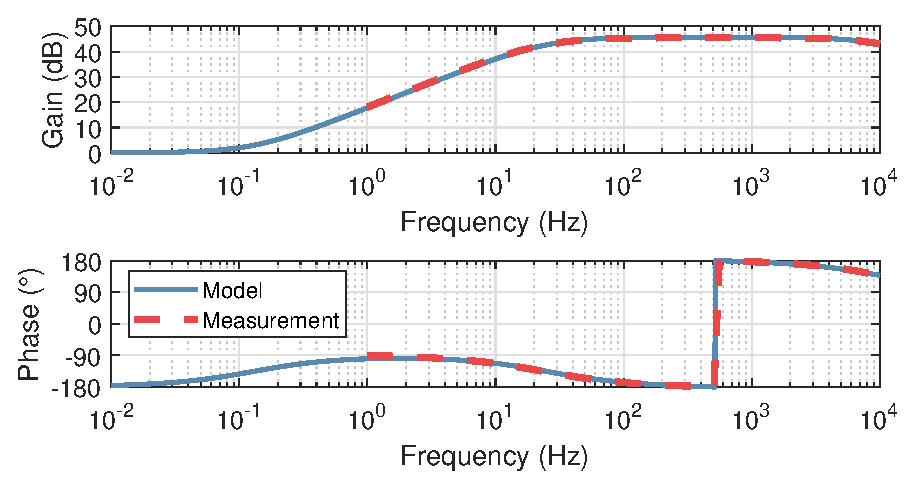
\includegraphics[width=1\linewidth]{Figures/MZ_chapter_in_air_send_recieve_filter}
	\caption{The transfer function of the electronics for sending, receiving and whitening the photodiode signal was modelled and measured. This gave the desired level of SNR to make shot noise limited measurements above $\sim200\,\rm{Hz}$.}
	\label{fig:mzchapterinairsendrecievefilter}
\end{figure}
\par
A servo was required to lock the Mach-Zehnder to $<1\%$ of a fringe. The circuit diagram for the servo is shown in Figure \ref{fig:mzinairservocircuit}. The phase between the two beams was actuated on with by moving one of the corner mirrors with a PZT. The error signal was obtained by subtracting the signals from the two photodiodes. The error signal was low pass filtered, and the corner frequency of the low pass filter was at 1\,Hz. The PZT needed to be driven with a high voltage ($\sim100\si{\volt}$), so a high voltage op amp (OPA454) was used in the final stage of the servo electronics. The PZT had a capacitance, so the output of the OPA454 was followed by a resistor to prevent the op amp oscillating. This corresponded to an additional corner frequency in the servo at $\sim8\,\si{\kilo\hertz}$. To prevent the servo oscillating due to this additional pole, the overall gain of the servo was controlled with a potentiometer. A way of injecting signals onto the PZT was included in the servo. 
\begin{figure}
	\centering
	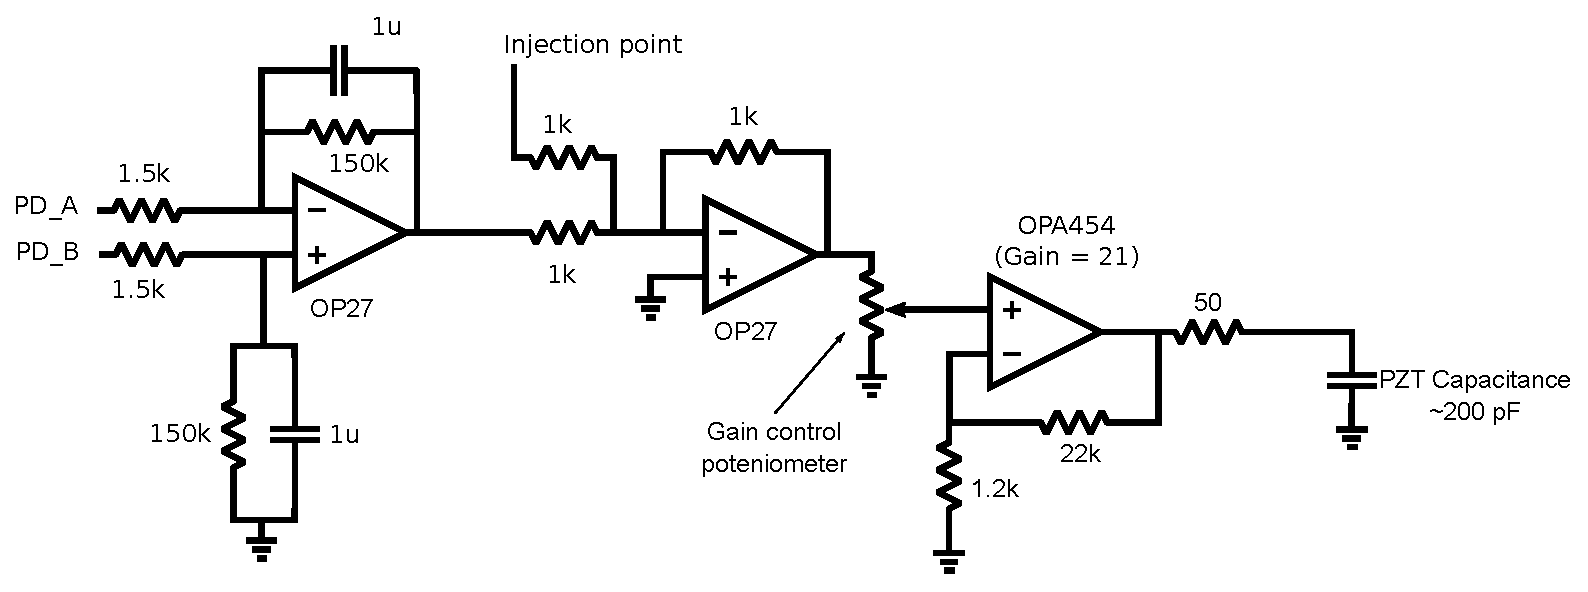
\includegraphics[width=1\linewidth]{Figures/MZ_in_air_servo_circuit}
	\caption{Circuit diagram for the electronics used to keep the in-air Mach-Zehnder locked to the middle of a fringe. The first stage subtracts the signals from the photodiodes and provides a 1\,Hz roll-off. The second stage allowed for a signal to be applied to the PZT. The final stage boosted the signal to around 100V. The final resistor was used to prevent the OPA454 oscillating.}
	\label{fig:mzinairservocircuit}
\end{figure}
\subsection{Calibration}
\label{sec:mz_chapter_in_air_cal}
The signal measured at the photodiodes can be calibrated in terms of the difference in path length between the two arms by applying a ramp signal to the PZT. Ramping the PZT causes the Mach-Zehnder to be driven over multiple fringes. The ramp signal and the photodiode signals were recorded on an oscilloscope. The difference in the photodiode signals was then plotted against the measured ramp signal. One period of this signal corresponds to one wavelength, so fitting a sinusoid to the data and finding its gradient around where the subtracted photodiode signal is 0\,V gives one the photodiode signal to path length conversion. This is shown in Figure~\ref{fig:mzchapterinaircalibration}. This measurement was affected by the quantisation noise of the oscilloscope.
\par
Alternatively, on can calibrate the differential path length signal by measuring the power in the two beams while they are not interfering (see Equation~(\ref{eq:bhdforligo_interference_at_a_beam_splitter})). The power of the LO beam was measured to be $20.3\pm0.1,\si{\milli\watt}$. Without the ND filter, the power of the signal beam was measured to be $18.3\pm0.1\,\si{\milli\watt}$, so with the ND filter it would be 78\,\si{\micro\watt}. This calibration is shown in Figure~\ref{fig:mzchapterinaircalibration}, and it agrees with the calibration obtained via ramping the PZT voltage to within 10\%.
\begin{figure}
	\centering
	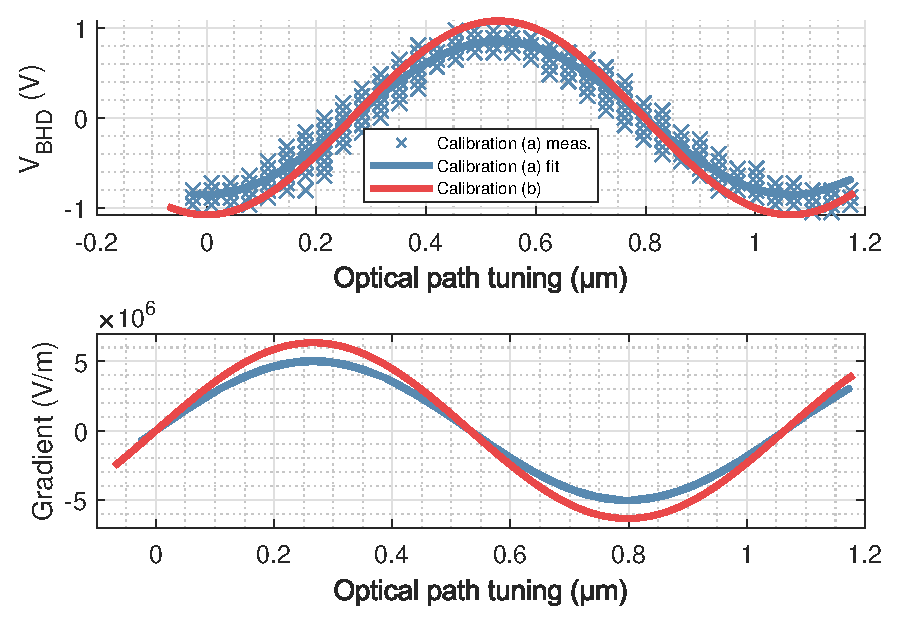
\includegraphics[width=1\linewidth]{Figures/MZ_chapter_in_air_calibration}
	\caption{There are two ways of calibrating the differential photodiode signal that will be generated by a change in optical path length between the two paths in the Mach-Zehnder. Method (a) is to measure a ramp signal that is applied to the PZT while simultaneously measuring the photodiode signals. The measurement of this is shown by the blue crosses, and the fit to this data is shown by the blue line. Method (b) is to measure the power in the local oscillator and signal beams when they are not interfering. From this, Equation~(\ref{eq:bhdforligo_interference_at_a_beam_splitter}) can be used to find the response of the Mach-Zehnder. This is shown by the red line. Thus, the blue and red data are independent of each other. The two calibrations agree to within 10\%. The gradient of $V_{BHD}$ is used to get the conversion factor for a change in beam power to a change in differential path length.}
	\label{fig:mzchapterinaircalibration}
\end{figure}
\subsection{Measurement of Shot Noise}
The Mach-Zehnder was locked, and the difference between the photodiode signals was measured. To demonstrate that the difference in the photodiode signals depended on the differential path length of the Mach-Zehnder, a modulation at 6033\,Hz was applied to the PZT. The amplitude spectral density of the difference in the photodiode signals is shown in Figure~\ref{fig:mzchapterfullnoisespectrum}. The signal was calibrated using the ramp technique described in Section~\ref{sec:mz_chapter_in_air_cal}. The dashed red line indicates the noise predicted by Equation~\ref{eq:MZ_chapter_shot_noise_level}, and at frequencies free of noise due to acoustic vibrations, this matches the measured noise to within 5\%. Thus, the measurement was limited by shot noise.
%\begin{table}
%	\centering
%	\begin{tabular}{|c|c|}
%		\hline
%		Parameter & Value \\
%		\hline
%		Nyquist Frequency & 32768\,Hz\\
%		Frequency Resolution & 10\,Hz \\
%		Effective Noise bandwidth & 15\,Hz\\
%		Number of Averages & 459 \\
%		\hline 
%	\end{tabular}
%\caption{A Hanning window was used to average the data and generate the amplitude spectral density. }
%\end{table}
\begin{figure}
	\centering
	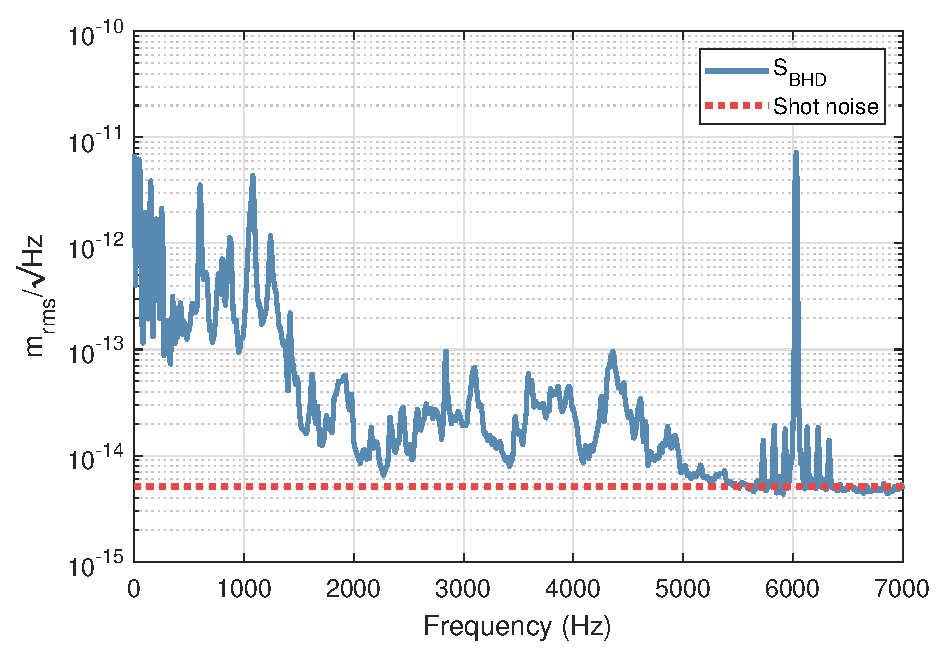
\includegraphics[width=1\linewidth]{Figures/MZ_chapter_full_noise_spectrum}
	\caption{The amplitude spectral density of the difference between the two photodiode's signals ($\rm{S_{BHD}}$) is shown in blue. The peak at 6033\,Hz was injected to demonstrate this measurement corresponds to differential arm length modulations. The expected shot noise is based on Equation~(\ref{eq:MZ_chapter_shot_noise_level}), and this is shown by the dashed red line. The noise measured at frequencies above 5500\,Hz is within 5\% of the expected shot noise. Below 5500\,Hz, acoustic noise limited the Mach-Zehnder's sensitivity.}
	\label{fig:mzchapterfullnoisespectrum}
\end{figure}
\section{Noise in an In-Vacuum Mach-Zehnder Interferometer and the Effect of Misalignment the Local Oscillator and Signal Beam}
\label{sec:MZ_chapter_in_vac}
To measure shot noise at frequencies around 100\,Hz, the frequency band of interest in a gravitational wave detector, the acoustic and seismic noise noise which shake the mirrors need to be reduced. This can be achieved by using suspended optics and performing the experiment in-vacuum. There was an opportunity to perform this experiment in-vacuum with left-over apparatus from a previous experiment. This proved challenging for as the interferometer was hard to lock due to large amounts of seismic motion coupling to the differential arm length. Ultimately, scattered light interfering with the differential arm signal meant that shot noise could not be measured at any frequency. However, this apparatus could be used to explore how misalignment will cause the signal to size to drop. 
\subsection{Apparatus for the In-Vacuum Mach-Zehnder}
A mach zehnder was constructed from suspended optics and placed in vacuum; this is shown in Figure \ref{}. The suspensions used were double pendulums of with masses of 75\si{\gram} separated by whiles of lengths 100\,mm (top to middle mass) and 150\,mm (middle to bottom mass), resulting in them having longitudinal resonances around $\sim 1$ \cite{Jans thesis}. The balanced homodyne readout platform (BHRP) was a suspended assembly that included the recombination beam splitter, steering mirrors for the recombined beams and photodiode. This photodiode circuit was the same as the one described in Section \ref{}. The vacuum system was pumped down to 1,mbar \ref{}. An NPRO was used to provide the laser light. 
\begin{figure}
	\centering
	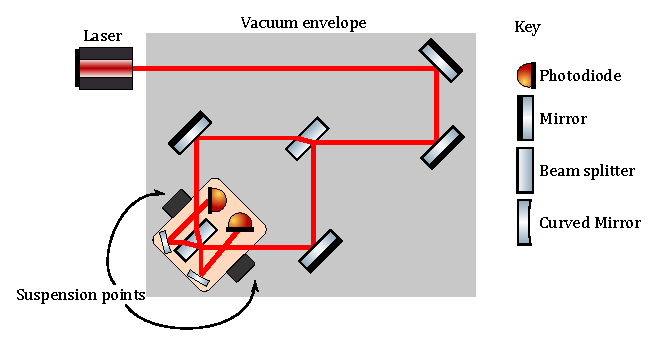
\includegraphics[width=1\linewidth]{Figures/MZ_chapter_in_vacuum_sketch}
	\caption{}
	\label{fig:mzchapterinvacuumsketch}
\end{figure}
\begin{figure}
	\centering
	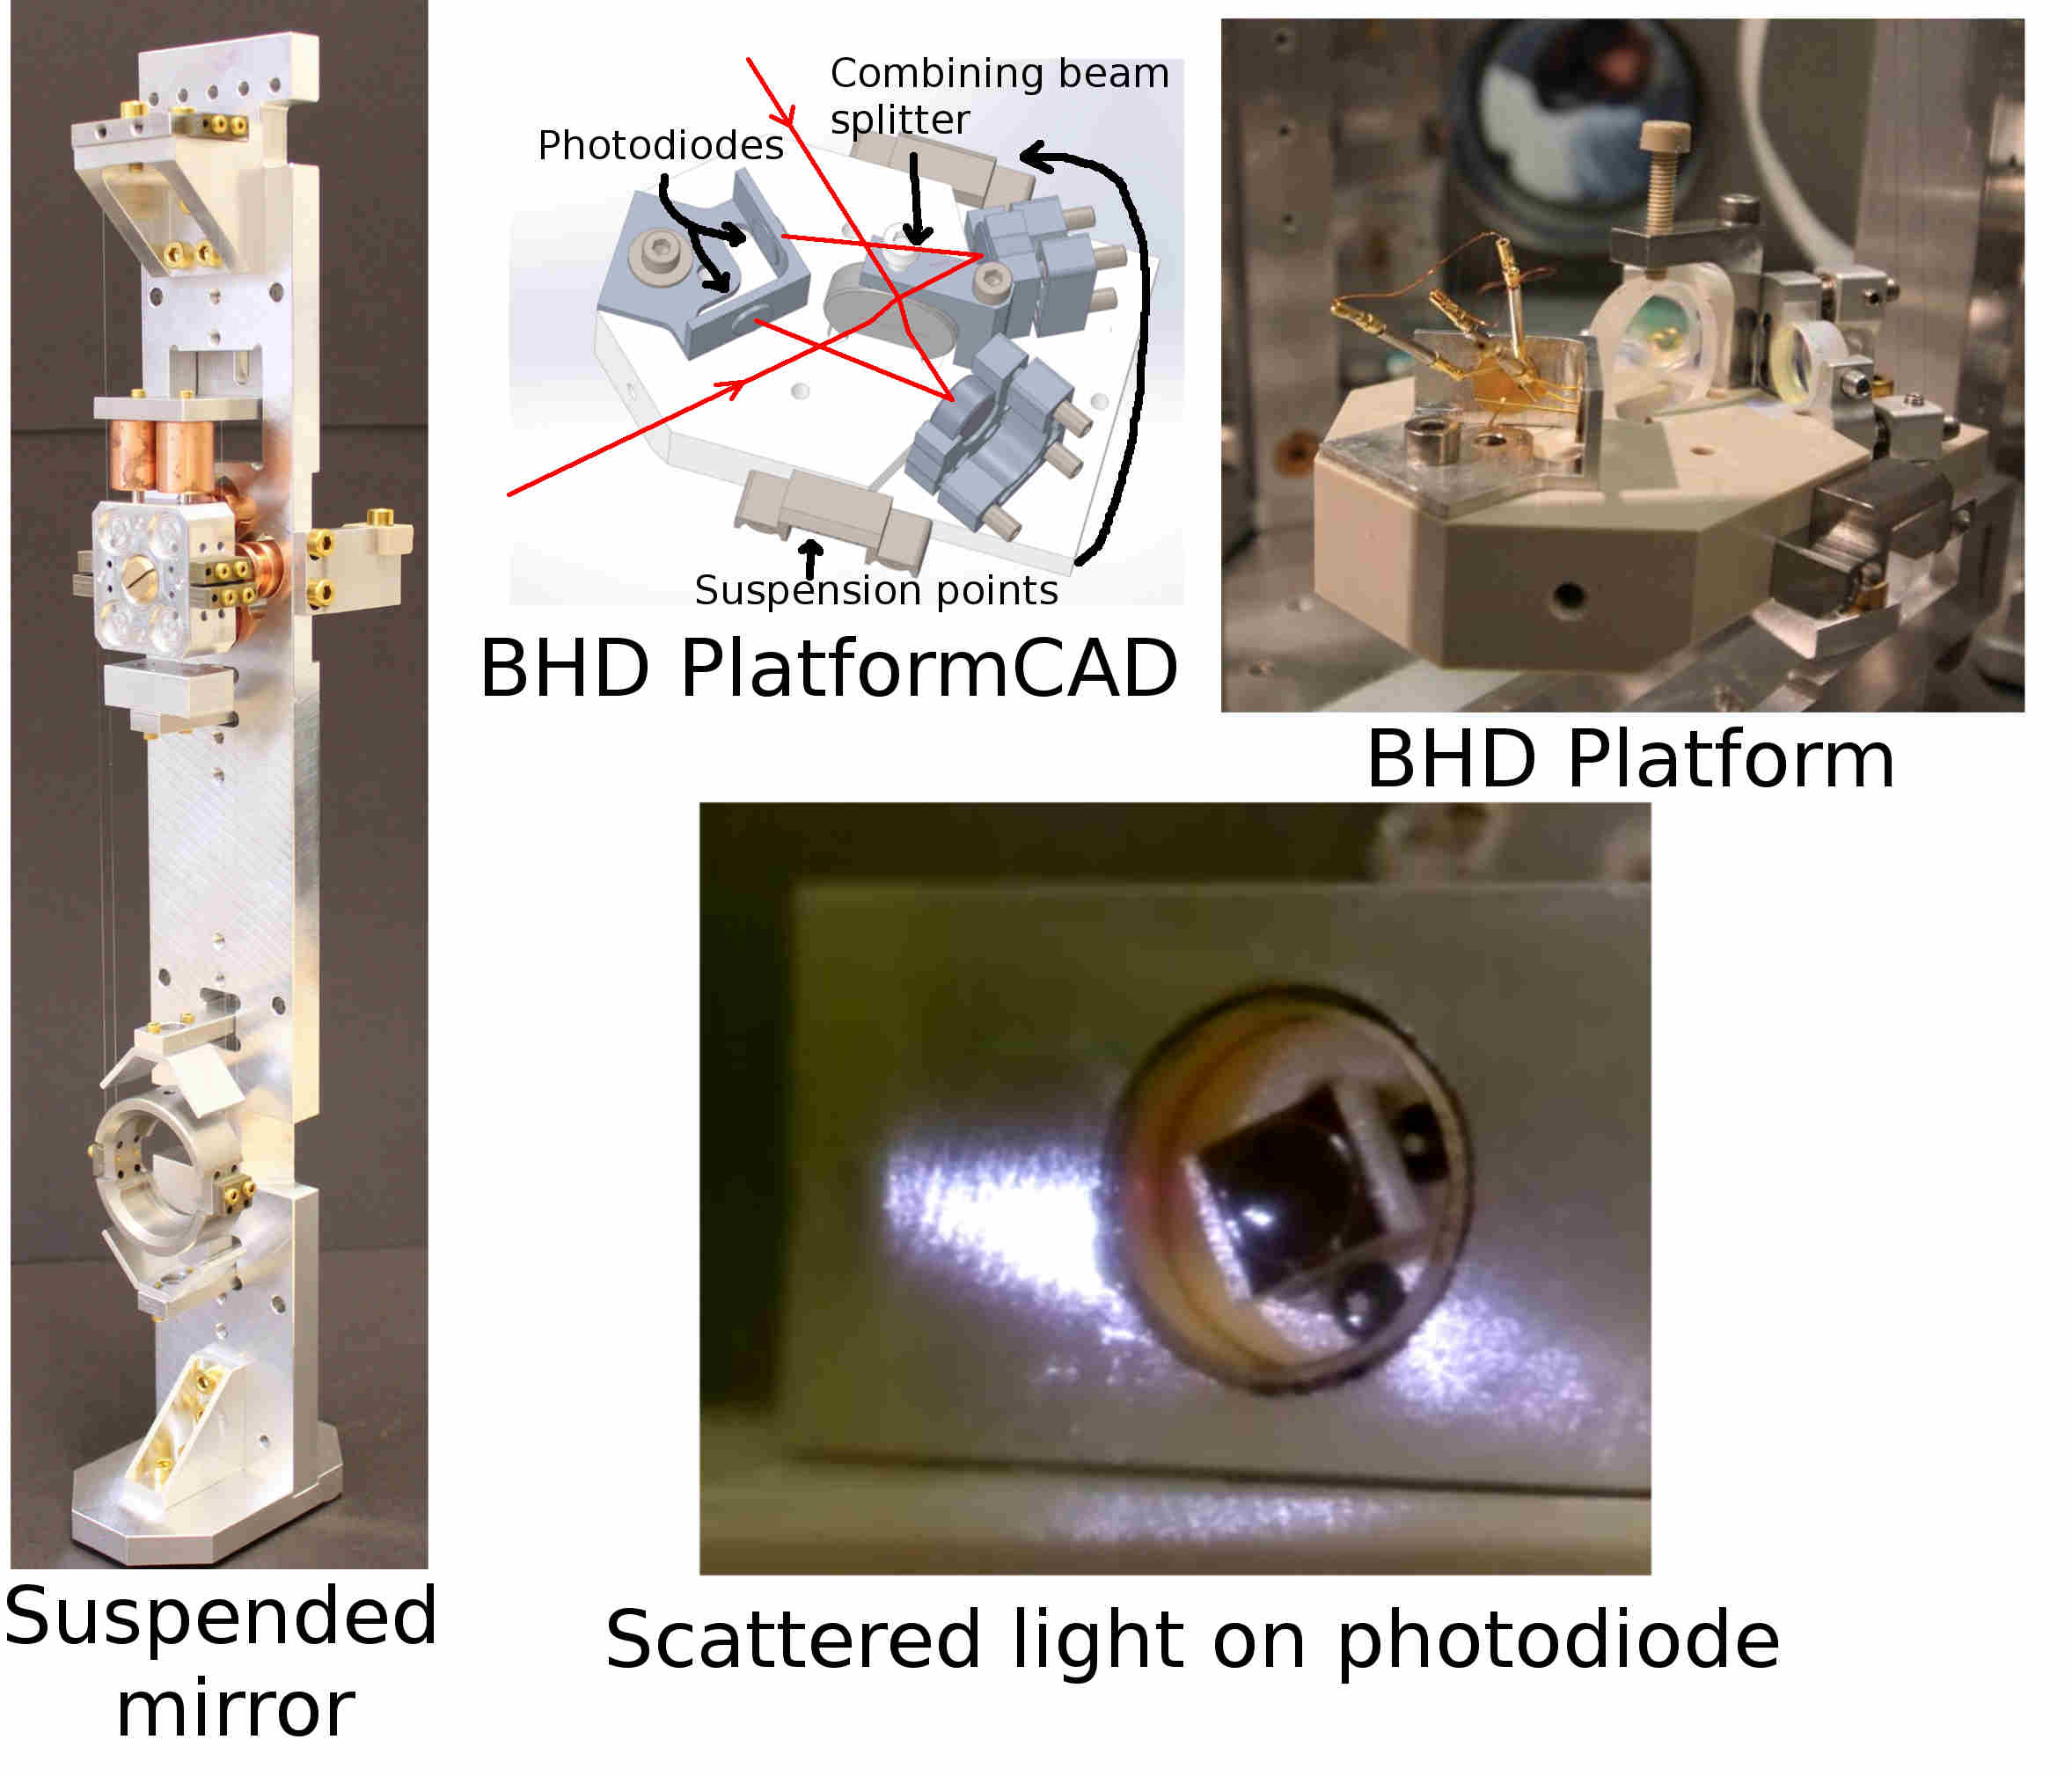
\includegraphics[width=1\linewidth]{Figures/MZ_chapter_in_vacuum_mz_apparatus}
	\caption{}
	\label{fig:mzchapterinvacuummzapparatus}
\end{figure}
\subsection{Calibration and Locking of the In-Vacuum Mach-Zehnder}
The differential arm length needed controlling below the suspension main resonance, ~ $\sim1$\,Hz as the optics moved on the order of one wavelength at these frequencies. Due to the design of the of the balanced homodyne readout, there are lots of suspension-related modes that couple to the longitudinal signal at around 30\,Hz. Additionally, the optical bench moved around a large amount due to poor seismic isolation. This meant that the differential arm length noise was at a similar level at $\sim30\,Hz$ as it was at $\sim1\,Hz$. 
\par
The suspended mirror was actuated on with a magnet+coil to lock the Mach-Zehnder arm length. The coil acted on a magnet glued to the bottom stage of the pendulum meaning that its strength fell as $1/f^2$ above the suspensions resonance. Thus, the coil would need to drive a large signal at $1$\,Hz, as well as one that was $~1000$ times greater at $\sim30$\,Hz. The magnet+coil strength was limited by geometry, e.g~ the size of the mirror, size of the magnet, size of the coil, amount of current that the coil could have etc., and so was not strong enough to do this. Therefore, the unity gain point needed a large gain at $\sim1$\,Hz while having a unity gain point limited to being below and $10$\,Hz by the suspension/coil driver actuator. To get the required gain, resonant gain filters were implemented in CDS, and to compensate for the phase problems these caused, phase compensation filters were made. \textcolor{red}{more detail?}
\par
The transfer function of the servo is shown in Figure \ref{fig:mzchapterflowdiagraminvacuumservo} and a sketch of the servo is shown in Figure \ref{fig:mzchapterflowdiagraminvacuumservo}. The servo consists of five logical blocks: the coil-driven suspended mirror, the `optical transfer function' that represents a change in differential arm length and the power of the recombined beam, the photodiode circuit, the analogue to digital/digital to analogue converters, and the digital filtering. The dewhitening filters were inverses of the whitening filter, and so they have no effect on the shape of the loop. As the transfer function of the suspension was simulated using the model developed in \ref{} and the digital filters just add shaping, to calibrate the loop, the conversion factors for the electronics and optics needed to be measured; this is summarised in table \ref{tab:MZ_chapter_servo_model}. 
\par
By injecting and measuring a signal across a `times one' block in the digital part of the servo, as the ratio of the two signals sizes gives the loop gain, the model's calibration was independently verified . This is shown in figure \ref{fig:mzchapterservotransferfunction}. This calibration ties up to within 0.1\,dB. Therefore, the unity gain point of the servo was at 5.5\,Hz with 15\si{\degree} of phase margin. 
\begin{table}
	\centering
	\begin{tabular}{|c|c|c|}
		\hline
		Component & Transfer function & unit \\
		\hline
		CDS DAC/ADC converters & 0.62 & mV/count\\
		Coil driver & 1.0 & mA/V \\
		Coil & 10 & mN/A \\
		Suspension & $H(f)$ & N/m\\ 
		Mach-Zehnder & 665000 & m/$\lambda$ \\
		Fringe to counts & 79000 & $\lambda$/count\\
		Digital filtering & $G(f)$ & count/count\\ 
		\hline
	\end{tabular}
\caption{Elements of the servo and their transfer functions. The suspension transfer function, $H(f)$, was obtained by simulation, the digital filter's transfer function is trivial, the coil's force per current was calculated using an existing script, the rest of the transfer functions were directly measured. These values were used to produce the servo model shown in Figure \ref{fig:mzchapterflowdiagraminvacuumservo}.}
\label{tab:MZ_chapter_servo_model}
\end{table} 
\begin{figure}
	\centering
	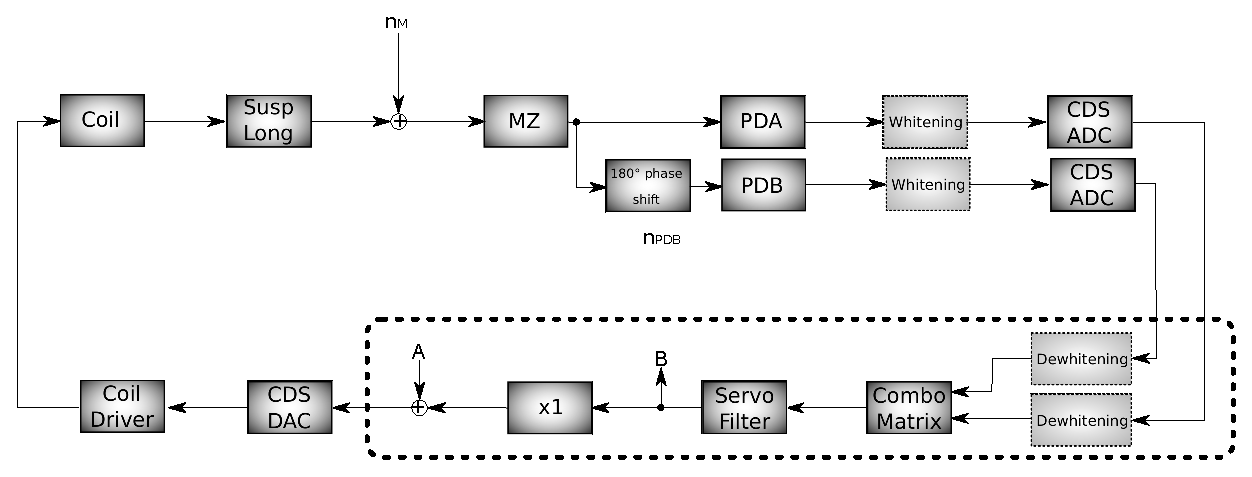
\includegraphics[width=1\linewidth]{Figures/MZ_chapter_flow_diagram_in_vacuum_servo}
	\caption{Flow diagram showing the each block of the servo used to lock the in-vacuum Mach-Zehnder. The digital part of the servo is shown in the dashed area. The injection points A and B were used to calibrate the servo (see Figure \ref{fig:mzchapterservotransferfunction} are around a times one block. The mirrors motion that the servo must correct for is represeted by the signal $n_M$. The information about the Mach-Zehnder differential arm length is encoded by two signals that are 180\si{\degree} out of phase. The whitening and dewhitening filters are paler as these do not affect the gain of the loop.}
	\label{fig:mzchapterflowdiagraminvacuumservo}
\end{figure}
\begin{figure}
	\centering
	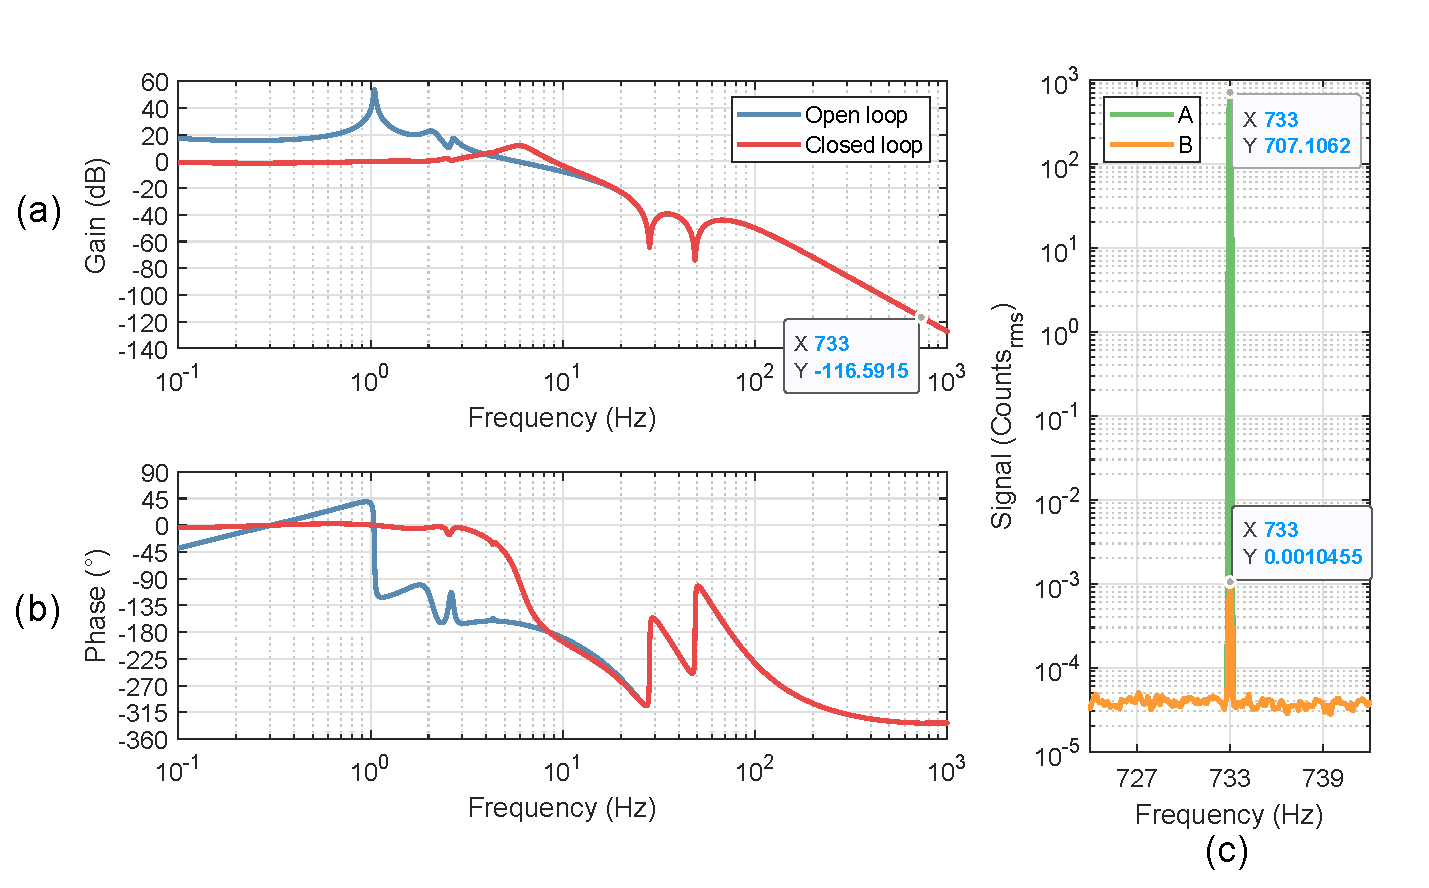
\includegraphics[width=1\linewidth]{Figures/MZ_chapter_servo_transfer_function_cali_combo}
	\caption{Panel (a) and Panel (b) is the Bode diagram of the Servo's open and closed loop transfer function. This was calibrated using the factors from \ref{tab:MZ_chapter_servo_model}. Panel (c) shows a measurement where a signal was injected at point A in the servo and measured at point B (see figure \ref{fig:mzchapterflowdiagraminvacuumservo}); these two points are separated by a times one block, and so the ratio of these signals represents the closed loop transfer function of the servo. These measurements are in agreement with the model to within 0.1\,dB.}
	\label{fig:mzchapterservotransferfunction}
\end{figure}
\subsection{Measurement of the Differential Arm Signal}
With the servo described in section \ref{}, the in-vacuum Mach-Zehnder was locked. The differential arm motion spectrum is shown in figure \ref{fig:mzchaptersuspendeddiffarm}. The curved steering mirrors used to guide the beam onto the photodiodes did not have an AR coating on their back face. This caused a large amount of scattered light. Scattered light generates a bilinear angle-to-intensity coupling. In an interferometer, this causes excess noise due to scattered light interfering with interferometers differential light mode. One of the great engineering achievements demonstrated at LIGO is the reduction of scattered light as this is currently a limiting source of noise at low frequencies. 
\begin{figure}
	\centering
	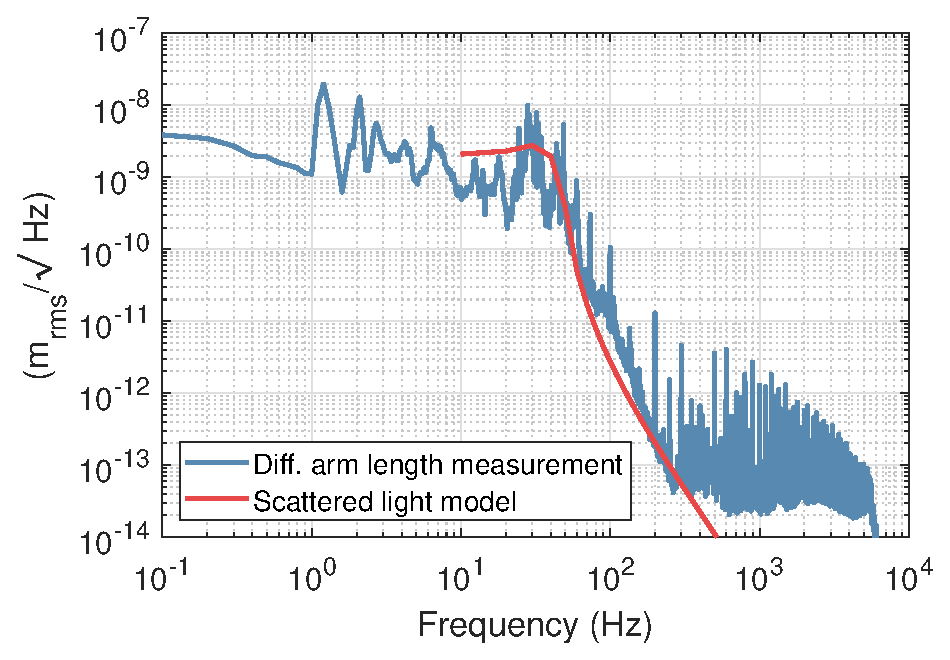
\includegraphics[width=1\linewidth]{Figures/MZ_chapter_suspended_diff_arm}
	\caption{Large amounts of scattering caused there to be a high amount of noise in the differential arm length signal's noise floor, this can be seen to limit the noise above $\sim200$\,Hz. The effect of the pendulums resonance at $\sim 1\,Hz$ was mostly removed by the servo but it can still be seen in the noise. Many suspension related peaks can be seen around 30\,Hz, these are due to the design of the BHD suspension. The $1/f^4$ slope is due to the suspension having two stages. For this measurement, shot noise would have been at $\sim 10^{-15}\,\rm{m}/\sqrt{\rm{Hz}}$.}
	\label{fig:mzchaptersuspendeddiffarm}
\end{figure}
\subsection{The Effect of Misalignment on the Size of a Signal in an Interferometer}
This apparatus can be used to verify that an angular misalignment, $\theta$, will cause the signal, $S$, to drop from its maximum value, $S_0$, as
\begin{equation}
S_{\rm{sig}} = S_0 e^{-\left( (\theta -\theta_0)/\theta_c\right)^2},
\label{eq:MZ_chapter_misalignment}
\end{equation}
where $\theta_c = \sqrt{2}\lambda_{\rm{EM}}/\pi w_0 $ is the characteristic angle of the a beam of waist $w_0$. The counts to angle was measured by applying the largest possible angle offset that CDS could provide and measuring the distance the beam moved, a few milimeter, over a distance of the order a metre. The beam's waist is know to be $\sim460\si{\micro\meter}$. A differential arm signal was generated and the resulting photodiode signal was measured for a range of angular misalignments. This result is shown in Figure \ref{fig:mzchaptermisalignmentplot}. To prevent noise at nearby frequencies from leaking into the measurement, a narrow frequency resolution was required (0.2\,Hz). Roughly 10 averages were made used to measure the signal size at each misalignment. The variance of these averages was large, this is represented by the error bars shown in figure \ref{fig:mzchaptermisalignmentplot}. A weighted non-linear least squares regression function (\textsc{Matlab}'s \texttt{nlinfit}) was used to fit the data to Equation \ref{eq:MZ_chapter_misalignment}, with each point weighted with $1/\rm{error}^2$. The resulting fit parameters were $S_0 = 6.9\pm0.3 \times10^{-3}$\,counts and $\theta_0 = 0.46\pm0.02\,\si{\milli\radian}$. The covariance between $S_0$ and $\theta_0$ was $\sigma_{S_0,\theta_c} = 2.4\times10^{-9}$ and the reduced $\chi^2$ statistic was 3.07.
\begin{figure}
	\centering
	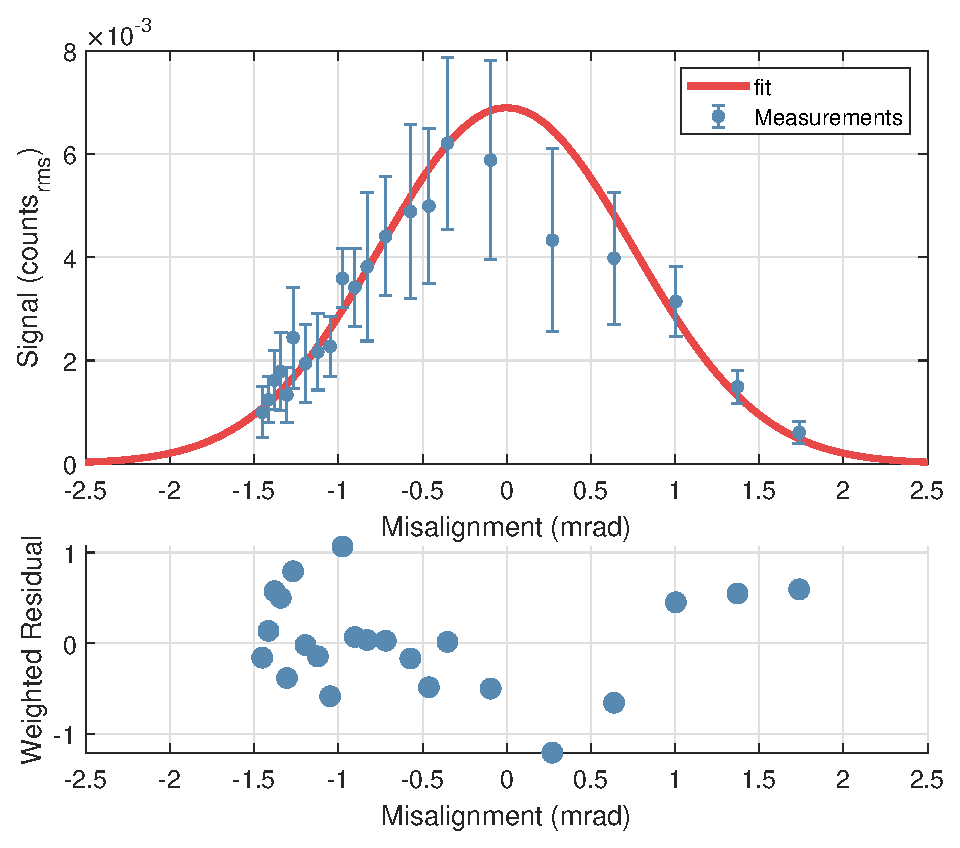
\includegraphics[width=1\linewidth]{Figures/MZ_chapter_misalignment_plot}
	\caption{Top panel: The in-vacuum Mach-Zehnder was misalignment. As the Mach-Zehnder was misaligned, there was less power in the HG00 mode. The decrease in power for a misalignment $\theta$ is  }
	\label{fig:mzchaptermisalignmentplot}
\end{figure}
\section{Conclusion}
A small, rigid mach zender was constructed to experimentally demonstrate the relationship between the local oscillators path length stability (see Equation \ref{eq:MZ_chapter_shot_noise_level}). This interferometer was calibrated and shot noise was measured. 
